% Author Vahid Partovi Nia
% Copyright Huawei Technologies
% Network Mind Team



\documentclass[12pt]{beamer}

\usetheme{Hannover}
\setbeamercolor{section in sidebar shaded}{fg=black}

\usecolortheme{beaver}
\beamertemplatenavigationsymbolsempty

%  \usebeamertemplate{navigation symbols}\hfill
%  \insertframenumber{}/\inserttotalframenumber}
  

\useoutertheme{sidebar}
\pgfdeclareimage[width=2.5\baselineskip]{institut-logo}{fig/mcgill_logo}
\setbeamertemplate{footline}
{\raisebox{-2ex}{\pgfuseimage{institut-logo}}
%  \hfill
\hspace{5cm}
  \usebeamertemplate{navigation symbols}
  \insertframenumber{}/\inserttotalframenumber
  \hspace{3.8cm}
YCBS255
}
%\setbeamertemplate{sidebar right}{}
  
\setbeamercolor{block title}{fg=darkred}
\setbeamercolor{local structure}{fg=darkred}

\setbeamercolor{palette sidebar secondary}{fg=darkgray, bg=white}



\usefonttheme{professionalfonts} % using non standard fonts for beamer


\makeatletter
\beamer@nav@subsectionstyle{hide/hide/hide}
\makeatother

\titlegraphic{
\includegraphics[width=2cm]{fig/mcgill_logo}}




\usepackage{listings}
\usepackage{xcolor}
\def \y {\mathbf y}
\def \X {\mathbf X}
\def \A {\mathbf A}
\def \t {^\top}
\def \inv {^ {-1}}
\def \x {\mathbf x}
\def \bbeta {\boldsymbol \beta}
\def \eeps {\boldsymbol \varepsilon}
\def \TV {\mathrm{TV}}
\def \Radio {\mathrm{Radio}}
\def \Newspaper {\mathrm{Newspaper}}
\def \Sales {\mathrm{Sales}}
\def \Balance {\mathrm{Balance}}
\def \Default {\mathrm{Default}}
\def \M {\mathcal{M}}
\def \r {\mathbf{r}}
\def \RSS {\mathrm{RSS}}


\definecolor{capri}{rgb}{0.0, 0.75, 1.0}
\definecolor{darkcyan}{rgb}{0.0, 0.55, 0.55}
\definecolor{deepfuchsia}{rgb}{0.76, 0.33, 0.76}
\begin{document}

% no title and no author on sidebar
\title[]{Model Selection and Shrinkage}   
\author[]{Vahid Partovi Nia} 
\institute{Lecture 05}
\date{}


\makeatletter
  \begin{frame}[plain]
    \hspace*{-\beamer@leftsidebar}%
    \advance\textwidth by \beamer@leftsidebar\relax
    \beamer@leftsidebar=\z@
    \begin{minipage}{\textwidth}\par%
      \maketitle
    \end{minipage}
  \end{frame}
  \makeatother



\frame{\frametitle{Outline}\tableofcontents} 

\setbeamertemplate{sidebar left}[sidebar theme]

\section{Credit dataset}
\frame{
\begin{itemize}
\item Credit dataset involves 11 attributes. The objective is to model 'Balance'. 
\item Available attributes are: Income, Limit, Rating, Cards, Age, Education, Gender, Student, Married, and Ethnicity.
\item Focus on quantitative variables: Income, Limit, Rating, Cards, Age, and Education.
\end{itemize}
}


\frame{\frametitle{Notation $n$ observation, $p$ features}
$\eeps = 
\begin{pmatrix} \varepsilon_1 \\ \vdots \\ \varepsilon_n  \end{pmatrix}, 
\y = \begin{pmatrix} y_1 \\ \vdots \\ y_n  \end{pmatrix}, 
\x = \begin{pmatrix} x_1\\ \vdots \\ x_p  \end{pmatrix}, 
\bbeta = \begin{pmatrix}  \beta_0 \\ \beta_1 \\ \vdots \\ \beta_p \end{pmatrix}$

$$\X_{n\times p} = \begin{pmatrix} \x_1\t \\ \vdots \\ \x_n\t \end{pmatrix} = \begin{pmatrix} 
x_{11} & x_{12}&  \ldots & x_{1p} \\
x_{21} & x_{22}&  \ldots & x_{2p} \\
\vdots & \vdots&  \ddots & \vdots \\
x_{n1} & x_{n2}&  \ldots & x_{np} \\
 \end{pmatrix}$$\\
 
 $$\X_{n \times (p+1)}=
 \begin{pmatrix} 
1 & x_{11}&  \ldots & x_{1p} \\
1 & x_{21}&  \ldots & x_{2p} \\
\vdots & \vdots&  \ddots & \vdots \\
1 & x_{n1}&  \ldots & x_{np} \\
 \end{pmatrix}
 $$
}


\frame{\frametitle{Matrix differentiation}
\begin{eqnarray*}
\y &=& \X\bbeta +\eeps \\
S(\bbeta) &=& (\y-\X\bbeta)\t (\y-\X\bbeta) 
\end{eqnarray*}
What is the minimizer of $S(\bbeta)$?
\pause
\begin{eqnarray*}
{\partial \X \bbeta \over \partial \bbeta   } =  \X\t \\
{\partial \bbeta \t \A \bbeta \over \partial \bbeta   } &=& (\A + \A\t )\bbeta
\end{eqnarray*}
}

\frame{\frametitle{Least squares}
\begin{eqnarray*}
\min && S(\bbeta) \\
{\partial S(\bbeta) \over \partial \bbeta}  &=& 0 \\
 (\X\t\X) \bbeta &=&  \X\t \y \\
  \bbeta &=& (\X\t\X)\inv \X\t \y 
\end{eqnarray*}
}

\frame{\frametitle{Quantitative attributes}
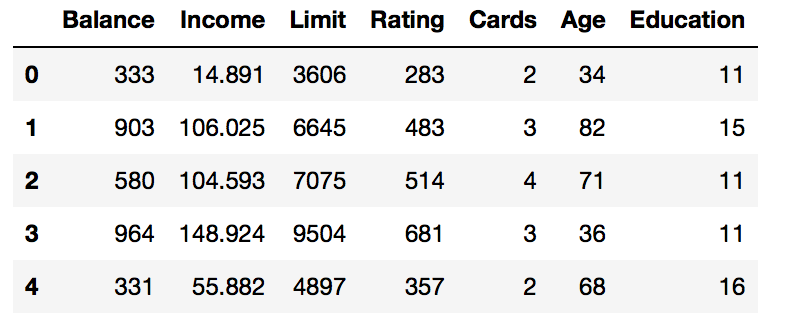
\includegraphics[width=\textwidth]{fig/credit_head}
}

\begin{frame}[fragile]\frametitle{Scatterplot Implementation}
\tiny	
\begin{lstlisting}
import pandas as pd
path='data/'
filename = path+'Credit.csv'
credit = pd.read_csv(filename)
credit = credit[['Balance','Income', 'Limit', 
	'Rating', 'Cards', 'Age', 'Education']]
credit.head()
\end{lstlisting} 
\begin{lstlisting}
from pandas.plotting import scatter_matrix
%matplotlib inline
scatter_matrix(credit, alpha=0.2);
\end{lstlisting} 
\end{frame}


\frame{\frametitle{Scatterplot}
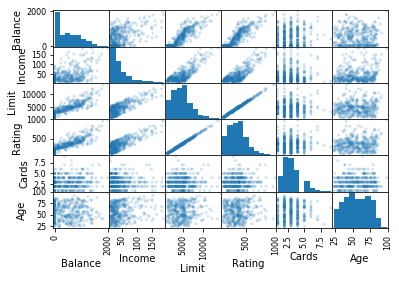
\includegraphics[width=\textwidth]{fig/credit_scatter}
}

\frame{\frametitle{Collinearity}
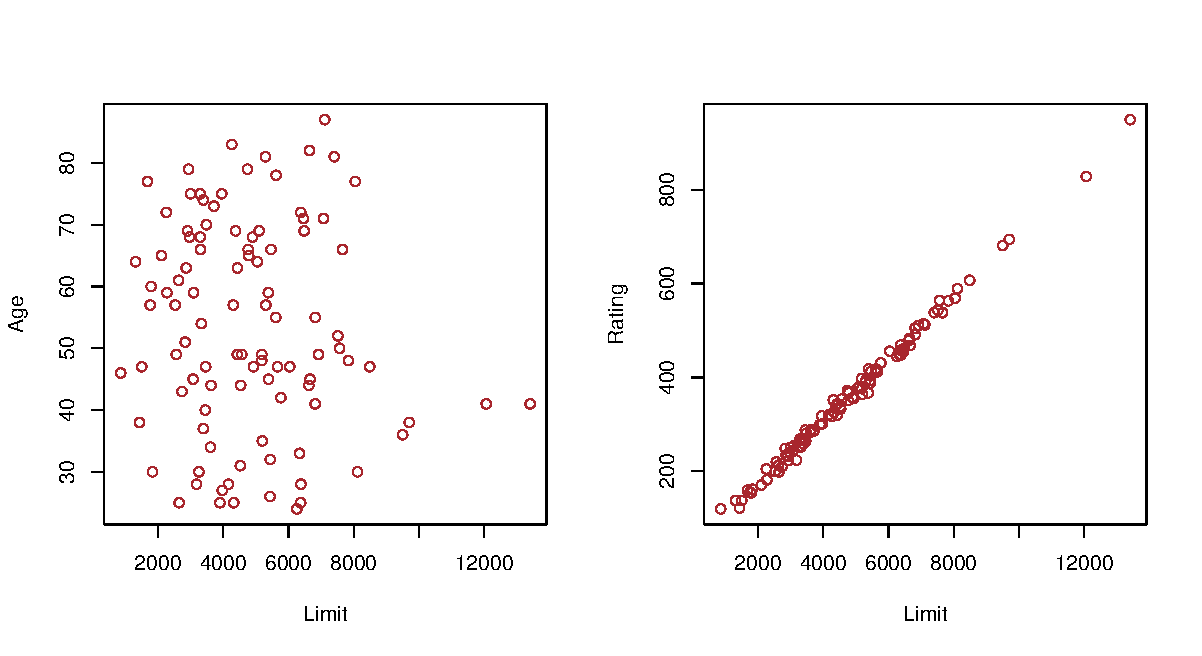
\includegraphics[width=\textwidth]{fig/3-14}
}


\frame{\frametitle{Effect of collinearity on estimation}
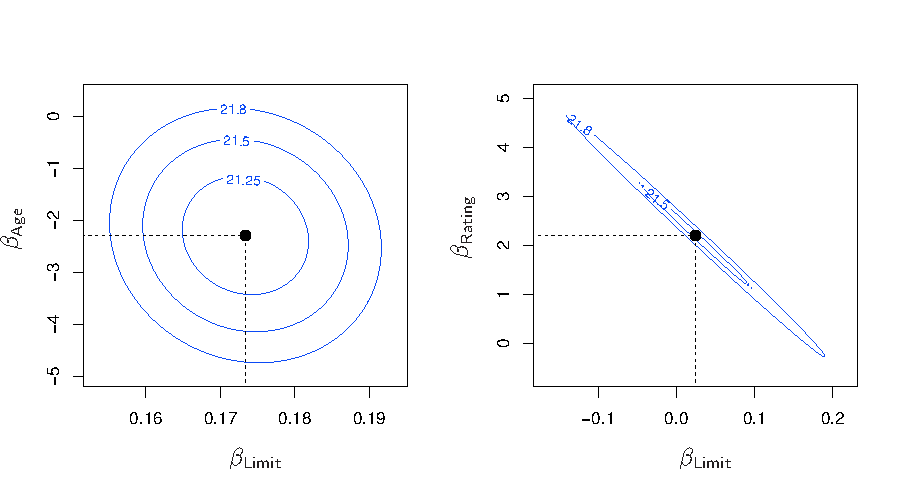
\includegraphics[width=\textwidth]{fig/3-15}
}

\frame{\frametitle{Effect of collinearity on estimation}
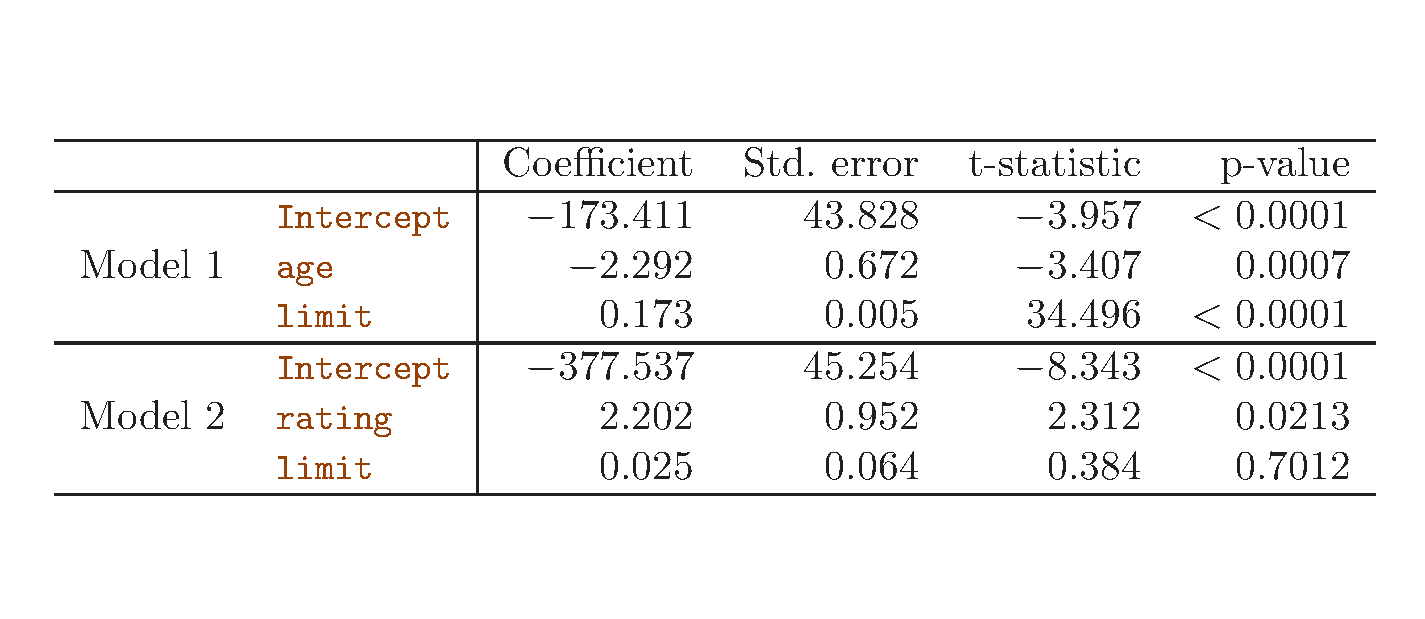
\includegraphics[width=\textwidth]{fig/tab_3-11}
}

\section{All subsets}
\frame{\frametitle{All possible subsets}
Suppose you have the response vector $\y$ and $\x_j , j=1,\ldots p$ attributes. 
\begin{itemize}
\item Fit $2^p$ possible models
\item Choose the model with the best AIC or BIC.
\end{itemize}
}

\section{Stepwise selection}

\frame{\frametitle{Forward}
Suppose you have the response vector $\y$ and $\x_j , j=1,\ldots p$ attributes. \\
Repeat the following algorithm until all attributes are in the model.
\begin{enumerate}
\item Initialize with the constant model $\y = \beta_0 $
\item Compute $\hat \y$
\item Compute the residual $\r = \y-\hat \y$
\item Find $j'$ the most correlated attribute $\x_j$ with $\r$.
\item Enter $j'$ to the model
\item Go to 2
\end{enumerate}
Select one of these models using AIC or BIC.
}

\section{Manual Implementation}

\begin{frame}[fragile]\frametitle{Model size = 1}
\tiny	
\begin{lstlisting}
from sklearn.linear_model import LinearRegression
y = credit['Balance'].values
X = credit[['Income']].values
lr = LinearRegression()
lr.fit(X,y)
score1 = lr.score(X,y)
\end{lstlisting} 
\pause
\begin{lstlisting}
y = credit['Balance'].values
X = credit[['Limit']].values
lr = LinearRegression()
lr.fit(X,y)
score2 = lr.score(X,y)
\end{lstlisting} 
\pause
\begin{lstlisting}
y = credit['Balance'].values
X = credit[['Rating']].values
lr = LinearRegression()
lr.fit(X,y)
score3 = lr.score(X,y)
\end{lstlisting} 
Which attribute you choose?
\end{frame}

\begin{frame}[fragile]\frametitle{Model size = 2}
\tiny	
\begin{lstlisting}
y = credit['Balance'].values
X = credit[['Rating', 'Income']].values
lr = LinearRegression()
lr.fit(X,y)
score31 = lr.score(X,y)
\end{lstlisting} 
\pause
\begin{lstlisting}
y = credit['Balance'].values
X = credit[['Rating', 'Limit']].values
lr = LinearRegression()
lr.fit(X,y)
score32 = lr.score(X,y)
\end{lstlisting} 
Which attribute you choose next?
\end{frame}



\frame{\frametitle{Credit data}
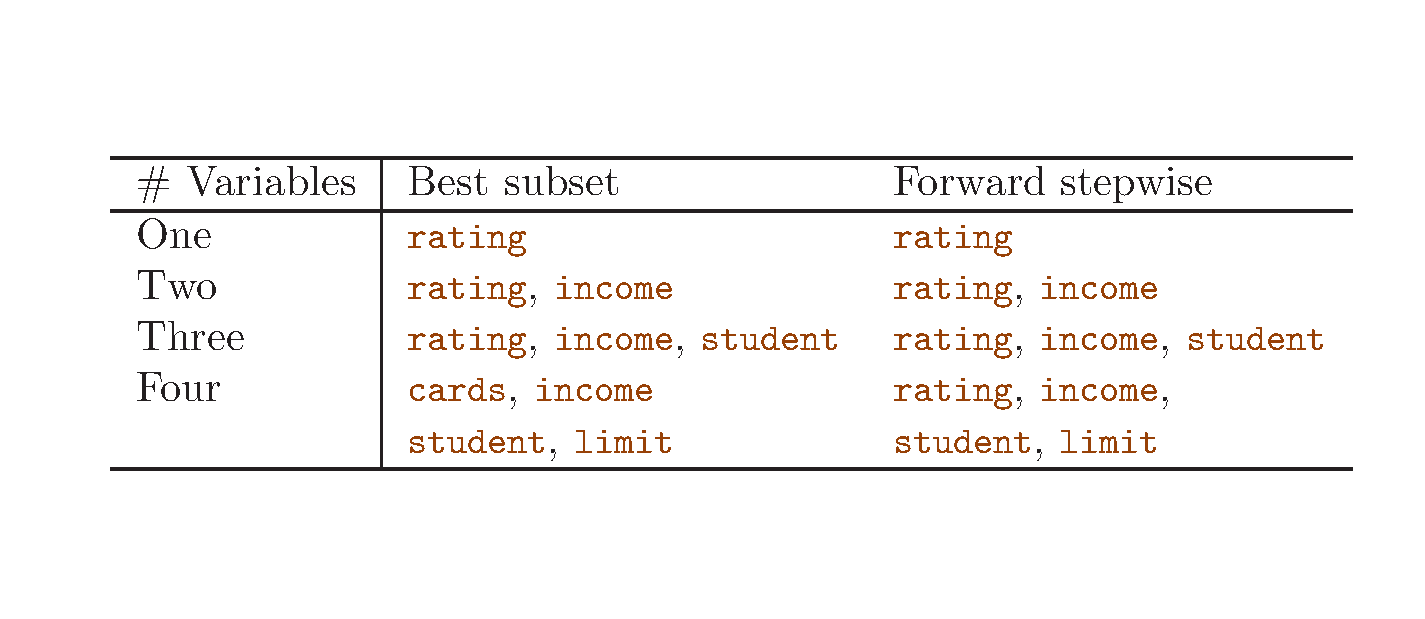
\includegraphics[width=\textwidth]{fig/tab_6-1}
}

\frame{\frametitle{Backward}
Suppose you have the response vector $\y$ and $\x_j , j=1,\ldots p$ attributes. \\
Repeat the following algorithm until there is no attribute in the model.
\begin{enumerate}
\item Initialize with the full $\y = \beta_0 + \beta_1\x_1 + \cdots \beta_p x_p $
\item Compute $\hat \y$
\item Compute the residual $\r = \y-\hat \y$ and $\RSS = \r\t\r$
\item Find $j'$ the attribute the drops $\RSS$ the least possible
\item Remove $j'$ from the model 
\item Go to 2
\end{enumerate}
Select one of these models using AIC or BIC.
}



\section{Shrinkage}
\frame{\frametitle{Least squares}
Least squares 
\begin{eqnarray*}
\hat\bbeta = \min  (\y-\X\bbeta)\t (\y-\X\bbeta) \\
\end{eqnarray*}
Subset selection 
\begin{eqnarray*}
\hat\bbeta &=& \min  (\y-\X\bbeta)\t (\y-\X\bbeta) \\
&\mathrm{s.t.}& \# \{\bbeta_j \neq 0\} \leq s
\end{eqnarray*}
or 
\begin{eqnarray*}
\hat\bbeta &=& \min  (\y-\X\bbeta)\t (\y-\X\bbeta) \\
&\mathrm{s.t.}& \sum_{j=1}^p I(\beta_j \neq 0) \leq s
\end{eqnarray*}
for a given model size $s$, where $I(.)$ is the indicator function.
}

\frame{\frametitle{Towards shrinkage}
for a given ball size $s$\\
Ridge regression
\begin{eqnarray*}
\hat\bbeta &=& \min  (\y-\X\bbeta)\t (\y-\X\bbeta) \\
&\mathrm{s.t.}& \sum_{j=1}^p \beta_j ^2 \leq s
\end{eqnarray*}
Lasso regression
\begin{eqnarray*}
\hat\bbeta &=& \min  (\y-\X\bbeta)\t (\y-\X\bbeta) \\
&\mathrm{s.t.}& \sum_{j=1}^p |\beta_j| \leq s
\end{eqnarray*}
}

\frame{\frametitle{Shrinkage versus selection}
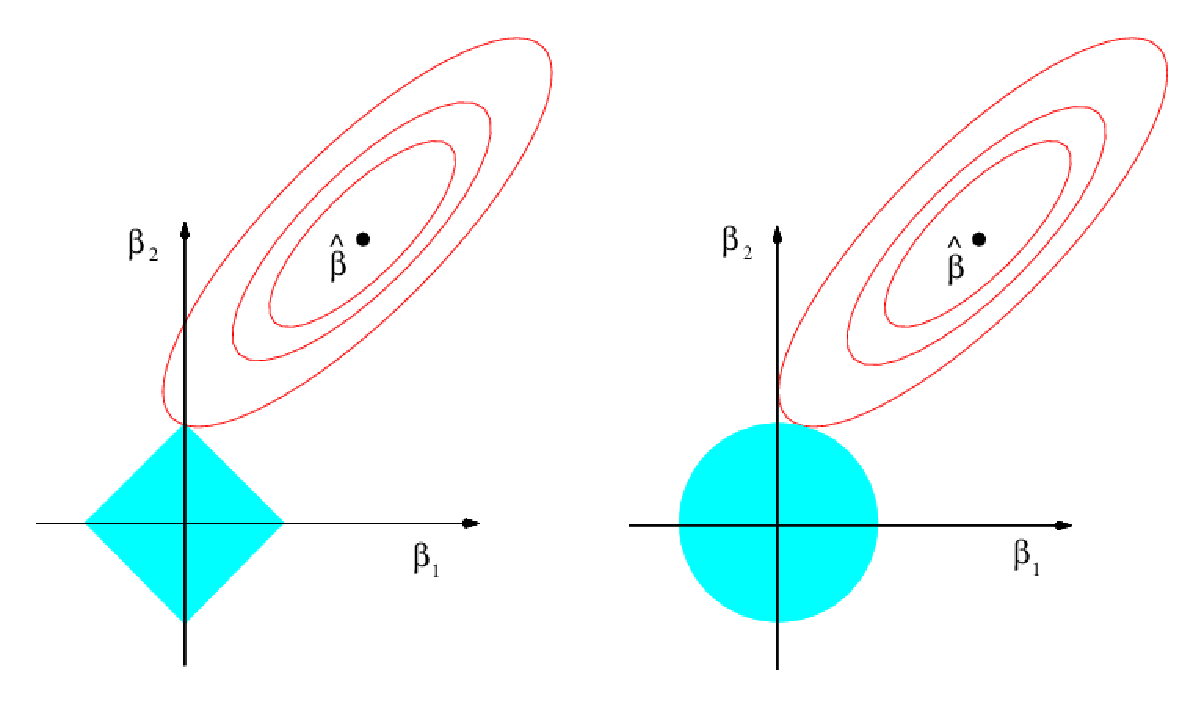
\includegraphics[width=\textwidth]{fig/6-7}
}

\frame{\frametitle{Lagrangian form}
For a given penalization constant $\lambda$\\
Ridge regression
\begin{eqnarray*}
\hat\bbeta &=& \min  (\y-\X\bbeta)\t (\y-\X\bbeta) + \lambda \sum_{j=1}^p \beta_j ^2 
\end{eqnarray*}
Lasso regression
\begin{eqnarray*}
\hat\bbeta &=& \min  (\y-\X\bbeta)\t (\y-\X\bbeta)+ \lambda \sum_{j=1}^p |\beta_j|
\end{eqnarray*}
}

\section{Ridge Implementation}
\begin{frame}[fragile]
\tiny
\begin{lstlisting}
from sklearn.linear_model import Ridge
import numpy as np
y = credit['Balance'].values
X = credit[['Income', 'Limit', 'Rating', 
	'Cards', 'Age', 'Education']].values
rr = Ridge(alpha=0, normalize=True)
rr.fit(X, y) 
\end{lstlisting}
\pause
\begin{lstlisting}
X_pred = np.array([15, 3000, 300, 2, 34, 16]).reshape(1,6)
rr.predict(X_pred)
\end{lstlisting}
\pause
\begin{lstlisting}
rr = Ridge(alpha=10, normalize=True)
rr.fit(X, y) 
rr.predict(X_pred)
\end{lstlisting}


\end{frame}


\begin{frame}[fragile]\frametitle{Ridge Generalized Cross-validation}
\tiny
\begin{lstlisting}
from sklearn.linear_model import RidgeCV
alpha_values = np.linspace(0.0001, 0.01, num= 100)
rrcv = RidgeCV(alphas=alpha_values, 
		normalize = True, store_cv_values = True)
rrcv.fit(X, y)
\end{lstlisting}
\begin{lstlisting}
import matplotlib.pyplot as plt
cv_values = np.sum(rrcv.cv_values_, axis=0)
plt.plot(alpha_values, cv_values, 'or');
\end{lstlisting}
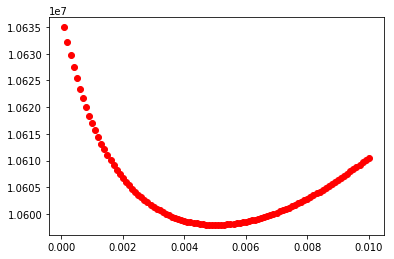
\includegraphics[width=0.4\textwidth]{fig/ridge_gcv}
\end{frame}

\section{Lasso Implementation}

\begin{frame}[fragile]\frametitle{Lasso}
\tiny	
\begin{lstlisting}
from sklearn.linear_model import Lasso
lr = Lasso(alpha = 0.1, normalize = True)
lr.fit(X,y)
lr.predict(X_pred)
\end{lstlisting} 
\pause
\begin{lstlisting}
from sklearn.linear_model import LassoCV
lrcv = LassoCV(alphas = alpha_values, cv = 10, normalize = True)
lrcv.fit(X, y)
lrcv.alpha_
\end{lstlisting} 
\end{frame}


\begin{frame}[fragile]\frametitle{Least Angle Regression}
The least angle regression provides a fast framework similar to forward selection gives the solution path for lasso.
{\tiny
\begin{lstlisting}
import matplotlib.pyplot as plt
from sklearn.linear_model import lars_path
alphas,_,coefs = lars_path(X, y, method='lasso', verbose=True)
alphas[1]
coefs[:,1]
\end{lstlisting} 
}
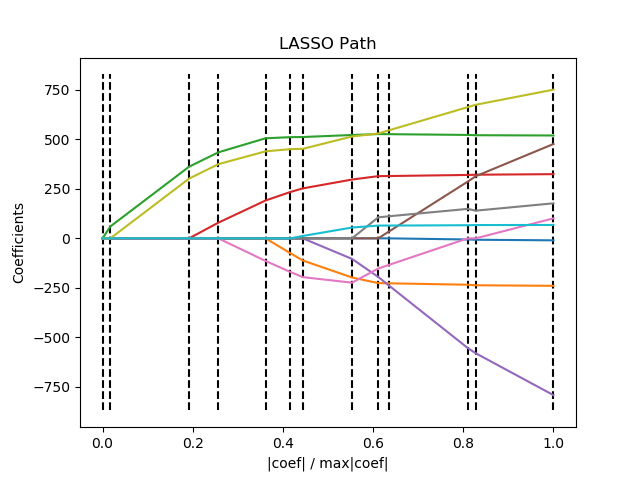
\includegraphics[width=0.5\textwidth]{fig/larspath}
\end{frame}

%\begin{frame}[fragile]\frametitle{}
%\tiny	
%\begin{lstlisting}
%\end{lstlisting} 
%\end{frame}

%\begin{frame}[fragile]\frametitle{}
%\tiny	
%\begin{lstlisting}
%\end{lstlisting} 
%\end{frame}


%}
%\frame{\frametitle{}
%\includegraphics[width=0.5\textwidth]{fig/}
%}
%
%
%
%

\end{document}
